% !TeX spellcheck = en_GB
\documentclass[10pt,letterpaper,oneside]{article}
\usepackage{fontspec}
\usepackage{arev}
\usepackage[utf8]{inputenc}
\usepackage[T1]{fontenc}
\usepackage{amsmath}
\usepackage{amsfonts}
\usepackage{amssymb}
\usepackage{graphicx}
\usepackage{csquotes}
\usepackage{booktabs}
\usepackage{multicol}
\usepackage{enumerate}
\usepackage{microtype}
\usepackage[labelfont=bf,font={small}]{caption}
\usepackage{hyperref}
\usepackage{booktabs}
\usepackage{subcaption}
\usepackage{fancyhdr}
\usepackage[svgnames]{xcolor}
\usepackage{mdframed}
\usepackage{multicol}
\usepackage[para]{footmisc}
\usepackage{siunitx}
\usepackage{cleveref}
\usepackage{listings}
\usepackage{cprotect}


\lstset{ % General setup for the package
	language=Python,
	basicstyle=\small\ttfamily,
	tabsize=4,
	columns=fixed,
	showstringspaces=false,
	showtabs=false,
	keepspaces,
	commentstyle=\color{SeaGreen},
	keywordstyle=\bf\ttfamily\color{DarkBlue}
}

\newfontfamily\symbolfont{Symbola}
\usepackage[left=1in,right=1in,top=1in,bottom=1in,marginparwidth=0.3in]{geometry}

\usepackage[sorting=none]{biblatex}
\addbibresource{../bibliography.bib}

\author{Andreas Stöckel\\[0.5cm]Based on lecture notes by\\Chris Eliasmith and Terrence~C.~Stewart}
\newcommand{\baseCodeURL}{https://github.com/astoeckel/syde556-w20/blob/master/lectures}

\fancyhf{}
\fancyhead[L]{SYDE 556/750 Lecture Notes}
\fancyhead[R]{Andreas Stöckel}
\fancyfoot[C]{\thepage}
\pagestyle{fancy}

\setlength{\parindent}{0em}
\setlength{\parskip}{0.5em}
\renewcommand{\baselinestretch}{1.25}
\renewcommand{\vec}[1]{{\mathbf{#1}}}
\newcommand{\mat}[1]{{\mathbf{#1}}}
\newcommand{\T}{\ensuremath{\mathrm{T}}}
\renewcommand{\epsilon}{\varepsilon}
\renewcommand{\phi}{\varphi}

\makeatletter
\newcommand{\superimpose}[2]{%
	{\ooalign{{#1}\hidewidth\cr{#2}\hidewidth\cr}}}
\makeatother
\newcommand{\SolidCircle}[2]{\superimpose{\color{#1}\symbolfont ⬤}{\textbf{\color{white}#2}}\hspace{1em}}
\newcommand{\OPlus}{\SolidCircle{DarkGreen}{\kern0.75pt+}}
\newcommand{\OMeh}{\SolidCircle{DarkOrange}{~}}
\newcommand{\OMinus}{\SolidCircle{DarkRed}{\kern2.25pt--}}

\newcommand{\YouTube}[2][Video]{\href{https://youtu.be/#2}{{\symbolfont 📺}~{#1}}%
%\footnote{\url{https://youtu.be/#2}}%
}

\newcommand{\CodeLink}[2][Code]{\href{\baseCodeURL/#2}{{\symbolfont ⌨}~\emph{#1}}}

\newcommand{\MakeTitle}[1]{
\maketitle
\begin{center}
	
\includegraphics[width=0.5\textwidth]{../assets/uwlogo.pdf}\\[1cm]
	{#1}\
\end{center}

\vfill

\thispagestyle{empty}
\setcounter{page}{0}
\newpage

\pagenumbering{roman}
\setcounter{tocdepth}{2}
\tableofcontents
\newpage

\setcounter{page}{0}
\pagenumbering{arabic}}

\reversemarginpar


\newcommand{\ColorBox}[3]{%
	\marginpar{%
		\huge\raisebox{-3ex}{\symbolfont{#1}}%
	}%
	\begin{mdframed}[hidealllines=true,backgroundcolor=#2,innertopmargin=0.25cm,innerbottommargin=0.25cm]%
		{#3}
	\end{mdframed}}

\newcommand{\Note}[1]{\ColorBox{📌}{WhiteSmoke}{\textbf{Note:} #1}}
\newcommand{\Example}[1]{\ColorBox{💡}{WhiteSmoke}{\textbf{Example:} #1}}
\newcommand{\Aside}[1]{\ColorBox{🌟}{WhiteSmoke}{\emph{Aside:} #1}}
\newcommand{\Python}[1]{\ColorBox{🐍}{WhiteSmoke}{#1}}
\newcommand{\Notation}[1]{\ColorBox{\huge$\Sigma$}{WhiteSmoke}{\textbf{Notaton:} #1}}

\newcommand{\ConstructionSite}{\hrulefill {\symbolfont 🚧} UNDER CONSTRUCTION {\symbolfont 🚧} \hrulefill}

\newenvironment{ImportantEqn}[1]{\mdframed\raggedleft\emph{({#1})}\align}{\endalign\endmdframed}

\date{February 13, 2020}
\title{SYDE 556/750 \\ Simulating Neurobiological Systems \\ Lecture 7: Temporal Basis Functions}


\begin{document}

\MakeTitle{\textbf{Accompanying Readings: See References}}

\section{Introduction}

\begin{figure}[h]
	\centering
	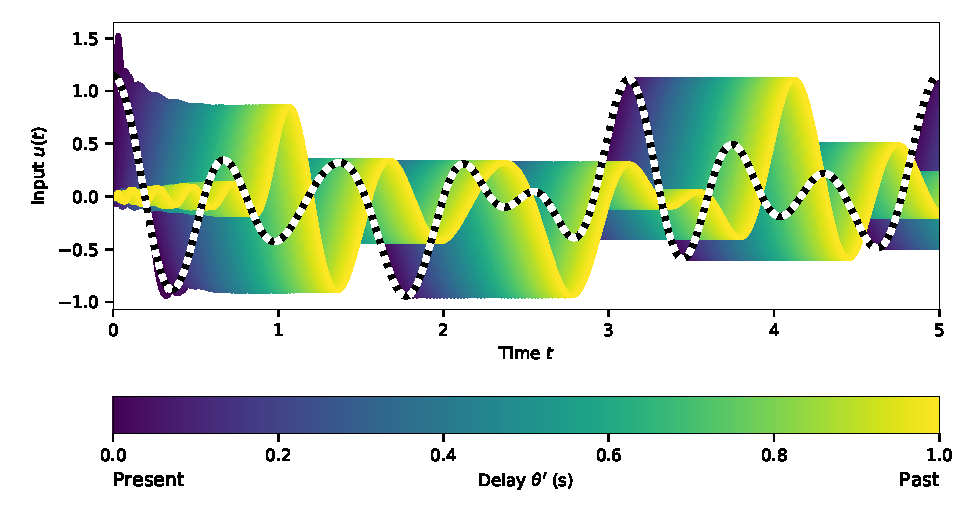
\includegraphics{media/delay_network_decoding.pdf}
	\caption{Example of the \enquote{delay network} we are going to discuss in the lecture. The dotted line is the input $u(t)$. The coloured lines correspond to delayed versions of the input signal. These delayed versions are all decoded from the same function representation $f_{[t - \theta, t]}(\theta')$. This diagram has been generated by decoding from a mathematically perfect implementation of the delay network. \CodeLink{lecture_06/media/code/delay_network_example.ipynb}}
\end{figure}

\Note{In this lecture we are going to discuss a very recent addition to the Neural Engineering Framework, the so called Delay Network developed by Aaron Voelker, first presented in \cite{voelker2018improving}, and discussed in more detail in his PhD thesis \cite{voelker2019thesis}. The Delay Network allows us to represent a function over time in a neural population. A more general version of the Delay Network has been presented at NeurIPS 2019 as the \enquote{Legendre Memory Unit}~(LMU)~\cite{voelker2019lmu}. The LMU can be used as a component within artificial Deep Neural Networks and vastly outperforms other recurrent architectures such as LSTMs in a variety of tasks.}

As humans, we often feel as if we have a good recollection of events that happened in the immediate past, where \enquote{immediate} refers to events happening within the last few seconds. As events move into the more distant past, it becomes increasingly harder to recall details. In this lecture, we are going to discuss a system that similarly memorizes stimuli, remembers them for a certain period, and then gradually forgets them.

Mathematically speaking, what we would like to have a function $f_{[t - \theta, t]}(\theta')$ which allows us to access stimuli $u(t)$ in a time-interval from $[t - \theta, t]$, that is
\begin{align*}
	f_{[t - \theta, t]}(\theta') = u\left(t - \theta' \right) \,, \text{where } 0 \leq \theta' \leq \theta \,.
\end{align*}
Put differently $f_{[t - \theta, t]}(0)$ will return the present stimulus $u(t)$, whereas $f_{[t - \theta, t]}(\theta)$ will return the input $\theta$ seconds from the past.

We would like to build a biologically plausible version of this system. That is, we would like to represent information about the immediate past in a population of neurons $f_{[t - \theta, t]}$. In order to do this, we have to solve two problems
\begin{enumerate}[1.]
	\item \textbf{Function representation.} So far we have seen how we can represent vectorial quantities in a neural population. But how can we represent an entire \emph{function} of the form $f_{[t - \theta, t]}(\theta')$ in a neural ensemble?
	\item \textbf{Updating the function representation.} If we were somehow able to represent functions in our neural population we still need to know how exactly to update this representation over time to get the de
\end{enumerate}

We discuss these two issues separately.

\section{Representing Functions}

\begin{itemize}
	\item \textbf{Idea:} We know how to represent vectors within a neuron population $\vec x$. Can we represent a function as a vector?
	\item Two approaches:
	\begin{itemize}
		\item Sampling/discretisation
		\item Basis functions
	\end{itemize}
\end{itemize}

\subsection{Sampling}

\begin{itemize}
	\item \textbf{Idea:} Measure the value of the function $f(t)$ at discrete points $x_1 = f(t_1), \ldots, x_N = f(t_N)$, where $t_i = \Delta t i$. Represent $x_1, \ldots, x_N$ as a vector $\vec x \in \mathbb{R}^N$.
	\item \textbf{Problem:} For a general function $f(t)$ in an interval we need infinitely many samples, even for a time-slice $[0, T]$. We cannot guarantee being able to perfectly reconstruct $f(t)$ with fewer samples.
	\item \textbf{The Nyquist-Shannon Sampling Theorem:} If $f(x)$ contains no frequencies greater than $B$ then it is \emph{completely} determined by samples spaced $\Delta t = \frac{1}{2B}$ apart ($N = 2BT$ equally spaced samples for a time-slice $[0, T]$). There is a \emph{one-to-one} mapping between the samples $\vec x$ and the function $f(x)$.
\end{itemize}

\subsection{Basis Functions}

\begin{itemize}
	\item \textbf{Idea:} $\hat f(t) = \sum_{i = 1}^q x_i \phi_i(t)$, where the $\vec \phi_i(t)$, are a set of \emph{basis functions}.
	\item The coefficients $\vec x = (x_1, \ldots, x_q)$ form a vector that could be represented in a neural ensemble.
	\item We can use a linear transformation to compute $f(t)$ at a single point $t$
	\begin{align*}
		f(t) &= \langle \vec a, \vec x \rangle \,, & \text{where } a_i &= \phi_i(t) \,.
	\end{align*}
	\item We can compute the $\vec x$ approximating a certain $f(t)$ by discretizing $f(t)$, $\vec \phi_1(t), \ldots, \vec \phi_q(t)$ and using least squares.
	\item Example Function Spaces
	\begin{itemize}
		\item Discrete Fourier Basis
		\item Discrete Cosine Basis
		\item Legendre Polynomials
		\begin{align*}
			\phi_i(t) = \tilde P_i(t) = (-1)^{i - 1} \sum_{k=0}^{i - 1} \binom{n}{k} \binom{n + k}{k} (-t)^{k}
		\end{align*}
		\item Neural Tuning Curves (this is exactly what we have done so far)
	\end{itemize}
	\item \textbf{Remark:} Sampling can be seen as a special case where $\phi_i(t) = \delta(t - \Delta t i)$.
\end{itemize}

\section{Representing the Past: The Delay Network}

\begin{itemize}
	\item \textbf{Motivation:} Implement a perfect delay of a time $\theta$ in the Neural Engineering Framework.
	\item This can be seen as a dynamical system. In the Laplace Domain, a perfect delay is $e^{-s\theta}$.
	\item Use Padé approximants up to a degree $q$ to compute an LTI system approximating $e^{-s\theta}$. This system has a one-dimensional input $u(t)$ and an internal state $\vec x(t)$ of dimension $q$:
	\begin{align*}
		\vec x(t) &= \mat A \vec x(t) + \mat B u(t) \\
	    \theta \mat{A} &= a_{ij} \in \mathbb{R}^{q \times q} \,, & \kern-0.5em a_{ij} &= \begin{cases}
		(2i + 1)(-1) & \kern-0.5em i < j \,,\\
		(2i + 1)(-1)^{i - j + 1} & \kern-0.5em i \geq j \,,
		\end{cases}\\
		\theta \mat{B} &= b_i \in \mathbb{R}^{q} \,, & \kern-0.5em b_i &= (2i + 1)(-1)^i \,.
	\end{align*}
	\item We can implement this LTI system as a neural ensemble using the transformation
	\begin{align*}
		\mat A' &= \tau \mat A + \mat I \,,\\
		\mat B' &= \tau \mat B \,.
	\end{align*}
	\item The state $\vec x \in \mathbb{R}^q$ represents more information than just the input $\theta$ seconds ago. It represents the state at every point in time up to $\theta$ seconds.
	\item In fact, $\vec x$ represents the function $f_{[t - \theta, t]}\left(\frac{\theta'}{\theta}\right) \approx u\left(t' - \theta' \right)$ in the Legendre basis
	\begin{align*}
		u\left(t' - \theta' \right) \approx f_{[t - \theta, t]}\left(\frac{\theta'}{\theta}\right) &= \sum_{i=1}^q \tilde P_i \left( \frac{\theta'}{\theta} \right) x_i(t) \,.
	\end{align*}
	\item When representing $\vec x$ in neurons, we can not only decode delays but any function using information from the past $\theta$ seconds.
	\item This network implements an optimal recurrent neural network remembering a slice of the past, as so called \enquote{reservoir}.
\end{itemize}

\printbibliography

\end{document}

